\documentclass[11pt,a4paper]{article}
\usepackage[T1]{fontenc}\usepackage[utf8]{inputenc}
\usepackage{lmodern,microtype,amsmath,amssymb,amsthm,mathtools}
\usepackage{booktabs,longtable,array,enumitem,xcolor,geometry,fancyhdr,hyperref,graphicx}
\geometry{margin=22mm}
\hypersetup{colorlinks=true,linkcolor=blue!55!black,urlcolor=blue,citecolor=blue!55!black,
 pdftitle={FIN ST1992--ST2081: Energy-Compatible Hodge Measure Classification, Schur No-Go and the Equivariant d1 Frontier},
 pdfauthor={Krzysztof Żuchowski}}
\pagestyle{fancy}\fancyhf{}\fancyhead[L]{FIN ST1992--ST2081}\fancyhead[R]{Release 11.06}\fancyfoot[C]{\thepage}\setlength{\headheight}{14pt}
\newtheorem{theorem}{Theorem}\newcommand{\status}[1]{\textsf{[#1]}}

\begin{document}
\begin{titlepage}\centering\vspace*{14mm}
{\Huge\bfseries FIN ST1992--ST2081\par}\vspace{4mm}
{\LARGE Energy-Compatible Hodge Measure Classification,\par}\vspace{2mm}
{\LARGE Schur No-Go and the Equivariant $d_1$ Frontier\par}\vspace{12mm}
{\Large Krzysztof \.Zuchowski\par}
{\normalsize Independent Researcher --- Fractal Information Theory Project\par}
{\normalsize ORCID: 0009-0002-0909-3613\par}\vspace{9mm}
{\large Six adaptive research rounds --- 90 programmes\par}
{\large Release 11.06 --- 1 September 2026\par}
\vfill
\begin{minipage}{.87\textwidth}\small
This report executes the highest-priority problem selected in Release 11.05:
classify positive face measures whose curvature energy is compatible with FIN
coarse/refinement maps.  The classification fixes inherited horizontal
weights but proves a growing vertical nonuniqueness.  A tensor-product Hodge
repair exists conditionally; the next exact decision problem is the full
$D_{12}$-equivariant second-differential classification.
\end{minipage}\vfill
{\small English mathematical and critical research report.}
\end{titlepage}

\begin{abstract}
ST1992--ST2081 classify diagonal face-curvature energies under the exact FIN
$12\to24\to48$ product refinement, test stronger naturality and tensor axioms,
and prove that Schur/minimal-extension consistency cannot determine the new
vertical face weights.

Fix a base face complex with curvature vector $F$ and energy
\[
E_0(F)=\frac12\sum_f\kappa_fF_f^2.
\]
Under $12\to24$, a coarse curvature embeds as two identical horizontal copies
and zero curvature on every edge-times-interval square.  Equality of fine and
coarse energy holds if and only if
\[
\kappa_{f,0}^{(24)}+\kappa_{f,1}^{(24)}=\kappa_f^{(12)}.
\]
Fiber-swap symmetry uniquely sets each inherited copy to $\kappa_f/2$.  All 66
new square weights remain arbitrary positive numbers; after $D_{12}$ symmetry
they form an $(\mathbb R_+)^6$ cone.  In unreduced coordinates the 220 energy
constraints leave an affine nullity of 286 among 506 fine face weights.

The classification iterates.  At $24\to48$, inherited base faces carry
$\kappa_f/4$, old square weights split into halves, and 144 new squares appear.
At least seven new natural square orbits are introduced, so after two steps the
vertical positive cone has dimension at least 13.  Exact mod-2 boundary ranks
show $H^1=0$ at all three product-cell levels, but no finite sequence of coarse
energy equalities selects future vertical weights.

Stronger elementary axioms do not resolve the ambiguity.  Positivity and joint
degree-one homogeneity admit geometric, harmonic, minimum and maximum rules.
Separate bilinearity in horizontal edge weight $w$ and fiber rate $q$ forces
only the shape
\[
\mu=cwq,
\]
leaving $c$, the base face set, base measure and gauge coupling free.

The Schur test gives a sharper no-go.  For one product square, write the coarse
horizontal mode as $a$, relative horizontal mode as $r$, and vertical-potential
difference as $s$.  The symmetric quadratic energy is
\[
E=\frac{k}{2}(a^2+r^2)+\frac{\mu}{2}(2r+s)^2.
\]
Minimizing over $(r,s)$ gives $r=s=0$ and
\[
E_{\min}(a)=\frac{k}{2}a^2,
\]
exactly independent of $\mu$.  Network-wide, identical layer connections and
flat fiber links give the same result.  Therefore no coarse classical energy,
energy-preserving embedding or minimal-extension Schur complement can identify
vertical Hodge weights.  Fine holonomy data or a quantum/fluctuation measure is
necessary.

A coherent conditional repair is available: given complete factor Hodge
inner products and a cellular product, the tensor-product inner product gives
cross-square weight proportional to $wq$ and is associative and positive.
It still inherits the unsolved base complex/measure, factor normalization,
$q$, differential-calculus quotient and overall action scale.  It is not a
bootstrap from $A$ alone.

The central no-go is therefore precise: energy preservation, positivity,
automorphism naturality, homogeneity, associativity and Schur consistency do
not select a unique Hodge measure.  The highest-value next theorem is to
classify all $D_{12}$-equivariant second differentials
$d_1:C^1\to C^2$ satisfying $d_1d_0=0$ and the $12\to24\to48$ refinement
intertwining relations.  A one-dimensional solution space after normalization
would be a major breakthrough; higher dimension would be a decisive strict
gauge-geometry no-go.
\end{abstract}

\tableofcontents\newpage

\section{Round I: ST1992--ST2006 --- $12\to24$ classification}

Let the selected base 2-complex have $N_2=220$ faces (the formulas apply to any
selected face family).  Its diagonal Hodge energy is
\[
E_0(F)=\frac12F^TM_0F,\qquad
M_0=\operatorname{diag}(\kappa_f)>0.
\]
The exact binary product refinement embeds coarse curvature as
\[
\iota F=(F,F,0_{66}),
\]
where the last block consists of new product squares.

Energy compatibility
\[
E_1(\iota F)=E_0(F)\quad\text{for all }F
\]
is equivalent coefficient by coefficient to
\[
\kappa_{f,0}+kappa_{f,1}=\kappa_f.
\]
Without fiber swap, each face has a free split
$(a_f\kappa_f,(1-a_f)\kappa_f)$.  Fiber-swap symmetry forces
\[
\kappa_{f,0}=\kappa_{f,1}=\frac12\kappa_f.
\]

Every new square has zero curvature on the coarse image, so its positive
weight is absent from the equality.  Thus the complete unreduced solution
space has 506 variables, 220 independent equations and nullity 286.  After
$D_{12}$ and fiber-swap reduction, the inherited triangle weights are fixed
but the six square-distance orbits remain:
\[
(\mu_1,\ldots,\mu_6)\in(\mathbb R_+)^6.
\]

A random 220-face curvature/weight replay verifies the energy identity exactly
to floating precision for arbitrary positive square weights.

\begin{theorem}[$12\to24$ energy-compatible measure classification]
Under diagonal face energy and fiber-swap symmetry, inherited horizontal face
weights are uniquely halved.  The six natural vertical square-orbit weights
are arbitrary positive parameters.
\end{theorem}

\section{Round II: ST2007--ST2021 --- iteration and associativity}

Exact product-cell enumeration gives:
\begin{longtable}{@{}p{.12\textwidth}p{.16\textwidth}p{.16\textwidth}p{.18\textwidth}p{.20\textwidth}@{}}
\toprule
Level & vertices & edges & 2-cells & cycle rank \\
\midrule\endhead
0 & 12 & 66 & 220 & 55 \\
1 & 24 & 144 & 506 & 121 \\
2 & 48 & 312 & 1156 & 265 \\
\bottomrule
\end{longtable}
Exact mod-2 boundary ranks are $(55,121,265)$, so the chosen product complexes
have $H^1=0$ at all levels.

At level two, the four copies of a base face carry $\kappa_f/4$.  Each old
level-one square splits into two copies of weight $\mu/2$.  Refining the 144
level-one edges creates 144 new squares.  Their natural edge types include at
least six base-distance horizontal types and one old-fiber vertical type.
Consequently the symmetric vertical measure cone has dimension at least
\[
6+7=13
\]
after two steps.

Direct four-copy refinement and iterated binary refinement agree on horizontal
quarters, so the positive inherited sector is associative.  Axis exchange can
relate some vertical weights only if the axes and rates are physically
equivalent; the free $q_1,q_2$ need not be.

By induction, every nontrivial refinement introduces new edge-times-interval
faces whose curvatures vanish on the prior coarse image.  No finite set of
coarse energy equalities can determine all future vertical weights.

\section{Round III: ST2022--ST2036 --- stronger axioms}

For a square generated by a horizontal edge weight $w$ and fiber rate $q$,
all of the following rules are positive and natural:
\[
wq,\qquad\sqrt{wq},\qquad\frac{2wq}{w+q},\qquad
\min(w,q),\qquad\max(w,q).
\]
The last four are jointly degree-one homogeneous and nonproportional on the six
strict distance classes.  Positivity, symmetry and degree-one homogeneity
therefore do not select a rule.

If one adds the stronger functional axiom that the rule is separately linear
in $w$ and $q$, then
\[
\mu(w,q)=c\,wq
\]
is forced.  This rule is associative under multiple product axes, with
cross-axis faces $c q_1q_2$.  However, the positive constant $c$ remains, as do
the base face set, base face measure and overall Wilson coupling.  The physical
dimensions of $w,q,\mu$ are not supplied, so the choice of homogeneity degree
is itself an assumption.

First-order factorization also has a normalization gauge: rescaling a factor
1-form inner product while compensating its differential preserves the same
0-form Laplacian but changes product 2-form normalization.

Thus bilinearity/associativity selects a useful conditional product
\emph{shape}, not a strict measure.

\section{Round IV: ST2037--ST2051 --- Schur no-go}

For one product square set
\[
a_0=a+r,\qquad a_1=a-r,
\]
and let $s$ be the difference of the two vertical potentials.  With equal
horizontal copy weights, the local energy is
\[
E(a,r,s)=\frac{k}{2}(a^2+r^2)+\frac{\mu}{2}(2r+s)^2.
\]
The exact stationarity equations yield
\[
r=0,\qquad s=0,\qquad
E_{\min}(a)=\frac{k}{2}a^2.
\]
The result contains no $\mu$.

The network generalization is immediate: copy the coarse connection to both
layers and set the fiber potential flat.  Every product-square curvature
vanishes.  The common vertical shift is a gauge zero mode and does not change
the conclusion.

\begin{theorem}[vertical Schur invisibility]
Under symmetric horizontal lifting, every positive vertical Hodge block gives
the same coarse minimal-extension Dirichlet/curvature energy.  Vertical face
weights cannot be inferred from coarse classical energy or its Schur
complement.
\end{theorem}

Breaking fiber-swap symmetry can make $\mu$ enter the reduced form, but violates
the earlier natural energy classification.  Gaussian fluctuation determinants
do depend on $\mu$; using them requires a path-integral measure, $\hbar$ or
temperature, regularization and counterterms.  Fine square holonomy or relative
mode observations can also measure $\mu$, but require an $OA$ instrument.

\section{Round V: ST2052--ST2066 --- monoidal Hodge repair}

Given complete factor 1-form Hilbert spaces and a cellular product, the tensor
product inner product supplies a coherent positive cross-square measure.  In a
normalized convention it yields
\[
\mu_e=w_e q.
\]
The construction is associative and compatible with horizontal energy
halving.  It is the best positive conditional repair found in this cycle.

It is not a bootstrap from $A$ alone:
\begin{itemize}
\item it inherits the unsolved base face set and measure;
\item factor inner-product normalizations and overall coupling remain;
\item $q$ and dimensional scale remain unsourced;
\item universal, clique, path and cubical calculi share $d_0$ but have different
      2-form spaces;
\item a noncommutative junk-form quotient depends on algebra representation and
      Dirac choice;
\item spectral-triple products require complete factor triples, gradings and
      real structures.
\end{itemize}

Thus the monoidal Hodge family is mathematically coherent only after the very
inputs the strict theory still needs to derive.

\section{Round VI: ST2067--ST2081 --- final classification}

\begin{longtable}{@{}p{.37\textwidth}p{.20\textwidth}p{.33\textwidth}@{}}
\toprule
Object & Status & Boundary \\
\midrule\endhead
horizontal weight halving & \status{Proven unique} & diagonal energy/fiber swap \\
vertical square weights & \status{Unconstrained cone} & coarse energy invisible \\
two-level associativity & \status{Proven horizontal} & vertical dimension $\ge13$ \\
bilinear product rule $cwq$ & \status{Conditional unique shape} & $c$/base/scale free \\
Schur/minimal extension selector & \status{Refuted} & exact $\mu$ independence \\
monoidal tensor Hodge & \status{Constructed conditional} & factor data supplied \\
unique strict Hodge measure & \status{Not established} & updated gate 0/7 \\
continuum gauge physics & \status{Not established} & locality/scale/OA absent \\
\bottomrule
\end{longtable}

The central theorem of the cycle is:
\[
\boxed{
\text{energy preservation fixes inherited horizontal weights but cannot fix
new vertical Hodge weights}.}
\]
The freedom is not a finite-level accident; it grows under iteration and lies
in the kernel of the coarse curvature embedding.

\begin{figure}[ht]
\centering
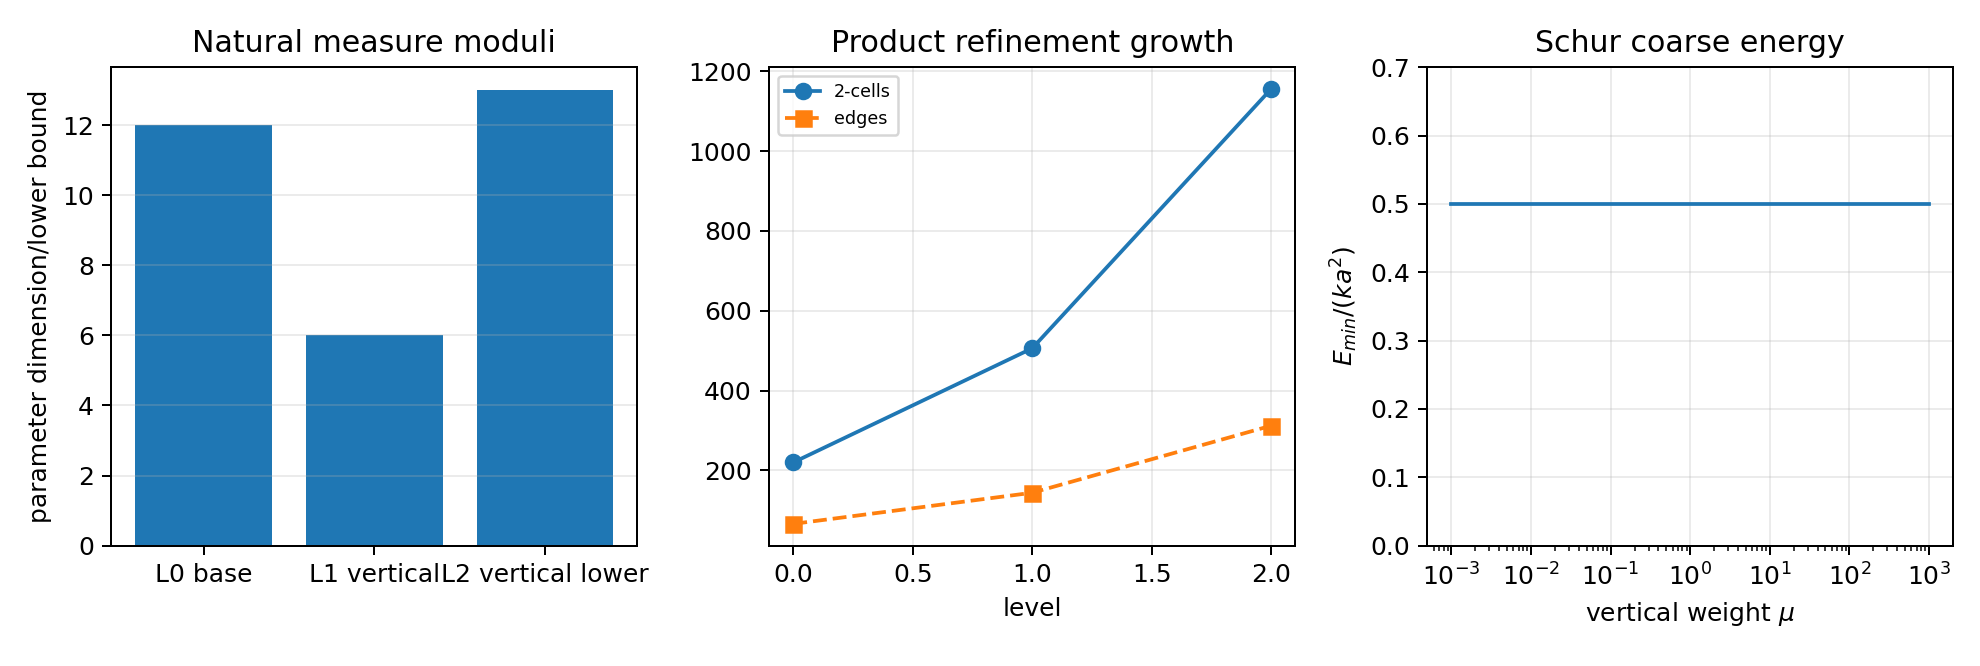
\includegraphics[width=.98\textwidth]{FIN_ST1992_ST2081_Figures/hodge_energy_classification.png}
\caption{Left: natural measure moduli.  Centre: growth of edges and 2-cells
through product refinement.  Right: minimized coarse square energy is constant
as the vertical Hodge weight varies.}
\end{figure}

\section{Highest-value next theorem}

Face-set and face-weight searches have reached a no-go under scalar energy
compatibility.  The next object must include the \emph{second differential}
itself.  The decisive finite problem is:
\begin{quote}
\emph{Classify all $D_{12}$-equivariant maps $d_1:C^1\to C^2$ satisfying
$d_1d_0=0$, positivity of a face inner product, and the $12\to24\to48$
refinement intertwining/coherence equations.  Determine the solution dimension
after quotienting overall scale and basis conventions.}
\end{quote}

The updated gate requires: an equivariant $d_1$, positive Hodge star,
$12\to24$ chain-map identity, $24\to48$ associativity, uniqueness modulo one
scale, continuum Maxwell scaling, and an $OA$ record.

This problem has high decision value because it is finite linear
representation theory before positivity/scaling.  A one-dimensional normalized
solution would be the first serious strict gauge-geometry candidate.  A higher-
dimensional solution space would be a decisive no-go for unique gauge geometry
from current FIN data.

\section{Route ranking}

\begin{longtable}{@{}p{.53\textwidth}p{.18\textwidth}p{.18\textwidth}@{}}
\toprule
Route & Rigorous-success estimate & Physics decision power \\
\midrule\endhead
$D_{12}$-equivariant $d_1$/refinement classification & 0.75 & 1.00 \\
conditional monoidal product Hodge model & 0.85 & 0.50 \\
quantum determinant selection of vertical weights & 0.30 & 0.65 \\
support-only face rules & 0.05 & 0.30 \\
$OA$ vertical-holonomy experiment & 0.40 & 0.55 \\
\bottomrule
\end{longtable}

These are strategic judgments, not empirical probabilities.

\section{Final interpretation}

\begin{quote}
FIN refinement has a coherent relative cellular and monoidal Hodge extension,
but coarse energy, symmetry, positivity and Schur consistency do not select its
vertical gauge geometry.  FIN remains a finite Dirichlet--Markov--spectral
information geometry with conditional gauge extensions, not a fundamental
physical theory.  The equivariant second-differential classification is now
the sharpest finite theorem capable of changing that verdict.
\end{quote}

\appendix
\section{Six-round ledger}
\begin{longtable}{@{}p{.18\textwidth}p{.35\textwidth}p{.37\textwidth}@{}}
\toprule
Range & Target & Verdict \\
\midrule\endhead
ST1992--ST2006 & $12\to24$ face energy & horizontal halves; vertical cone \\
ST2007--ST2021 & $24\to48$ associativity & quarters plus growing moduli \\
ST2022--ST2036 & stronger axioms & product shape conditional \\
ST2037--ST2051 & Schur/minimal extension & vertical-weight no-go \\
ST2052--ST2066 & monoidal Hodge & coherent conditional family \\
ST2067--ST2081 & synthesis & equivariant $d_1$ frontier \\
\bottomrule
\end{longtable}

\section{Reproducibility}
The authoritative result sets run from
\path{FIN_ST1992_ST2006_Results.json} through
\path{FIN_ST2067_ST2081_Results.json}.  Each contains fifteen programmes and
packet SHA-256 references.  The combined test
\path{test_fin_st1992_st2081.py} verifies all ninety packets, energy identities,
product-cell ranks, vertical cone counts, Schur independence, updated gate,
figure and nonpromotion boundaries.

\section{Nonclaims}
This report does not derive $d_1$, a unique face measure, gauge coupling,
continuum dimension, Maxwell normalization, physical scale, state ontology,
platform or evidence.  It does not complete legacy role transfer, QW-2191,
Standard Model, gravity, $L_{\rm total}$ or Theory of Everything.  All future
FIN PDFs remain English.

\begin{thebibliography}{9}
\bibitem{desbrun} M. Desbrun et al., Discrete Exterior Calculus, arXiv:math/0508341.
\bibitem{hatcher} A. Hatcher, \emph{Algebraic Topology}, Cambridge University Press.
\bibitem{rothe} H. J. Rothe, \emph{Lattice Gauge Theories}, World Scientific.
\end{thebibliography}
\end{document}
